% experiment_results.tex
En esta sección se presentan y discuten los resultados obtenidos en las mediciones empíricas. Para el análisis de complejidad, se han seleccionado gráficas en escala logarítmica para ambos ejes, lo que permite visualizar las diferencias en las tasas de crecimiento de los distintos algoritmos evaluados.

\subsection{Algoritmos de Ordenamiento}

Para analizar el rendimiento práctico del ordenamiento, la Tabla \ref{tab:sorting_summary} resume los tiempos promedio de ejecución para la instancia más grande evaluada ($n = 10^7$).

\begin{table}[H]
\centering
\caption{Tiempo de ejecución promedio (ms) para $n = 10^7$.}
\label{tab:sorting_summary}
\begin{tabular}{lrrr}
\hline
\textbf{Algoritmo} & \textbf{Aleatorio} & \textbf{Ascendente} & \textbf{Descendente} \\
\hline
Merge Sort & 11825.20 & 10048.85 & 9980.79 \\
Patience Sort & 8648.03 & 11235.24 & 2505.78 \\
\texttt{std::sort} & 2051.06 & 1244.50 & 1151.65 \\
\hline
\end{tabular}
\end{table}

Como se observa en la Tabla \ref{tab:sorting_summary}, \texttt{std::sort} supera holgadamente a las implementaciones manuales, siendo entre 4 y 5 veces más rápido. Esto demuestra el profundo nivel de optimización de la Standard Template Library (STL) de C++. Además, es notable la sensibilidad de Patience Sort a la distribución inicial: es significativamente más veloz en arreglos descendentes comparado con los ascendentes.

Para evaluar el crecimiento asintótico, la Figura \ref{fig:sorting_growth} presenta la evolución temporal del ordenamiento bajo escenarios de entrada aleatoria y ascendente.

\begin{figure}[H]
    \centering
    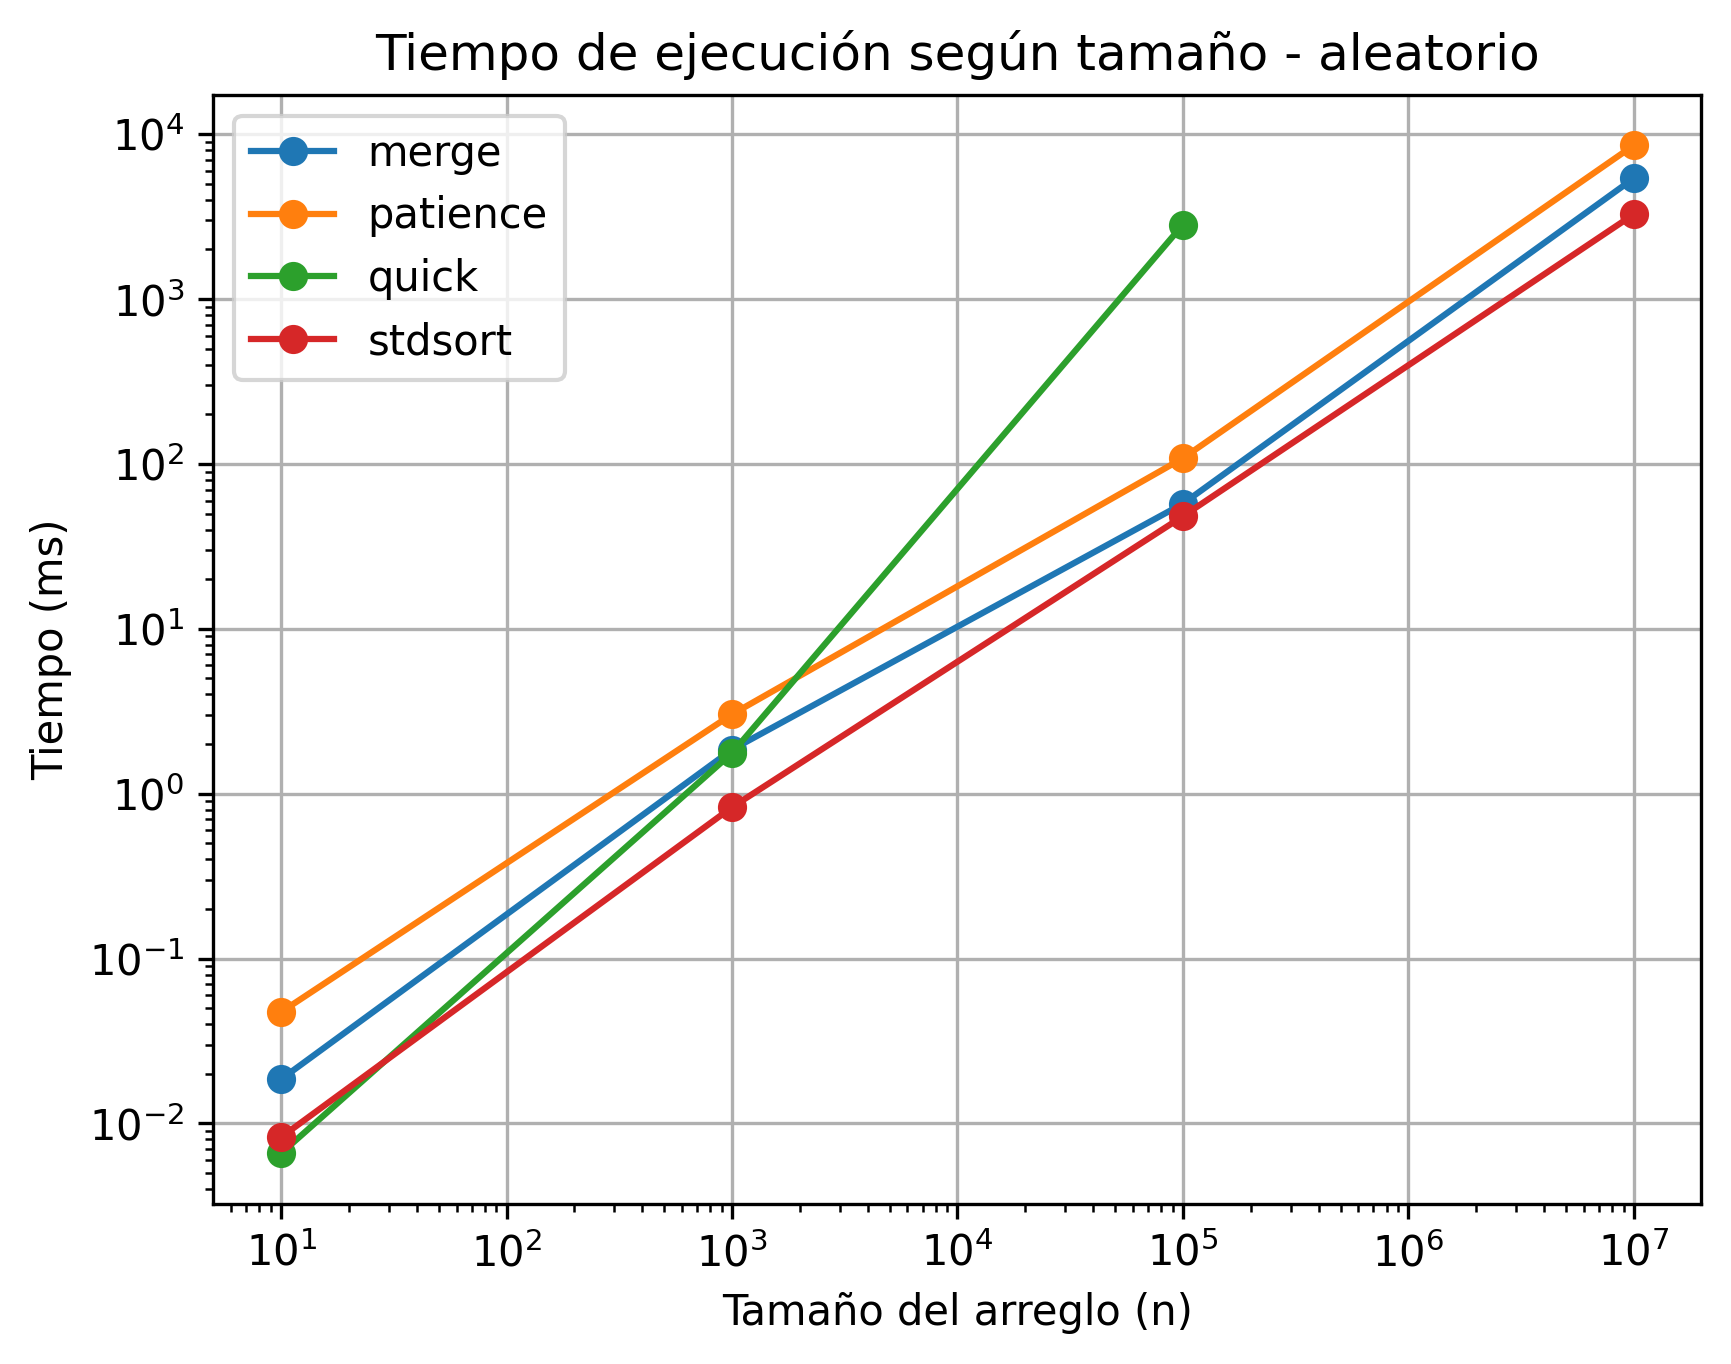
\includegraphics[width=0.48\textwidth]{../code/sorting/data/plots/sorting_tiempo_vs_n_aleatorio.png}
    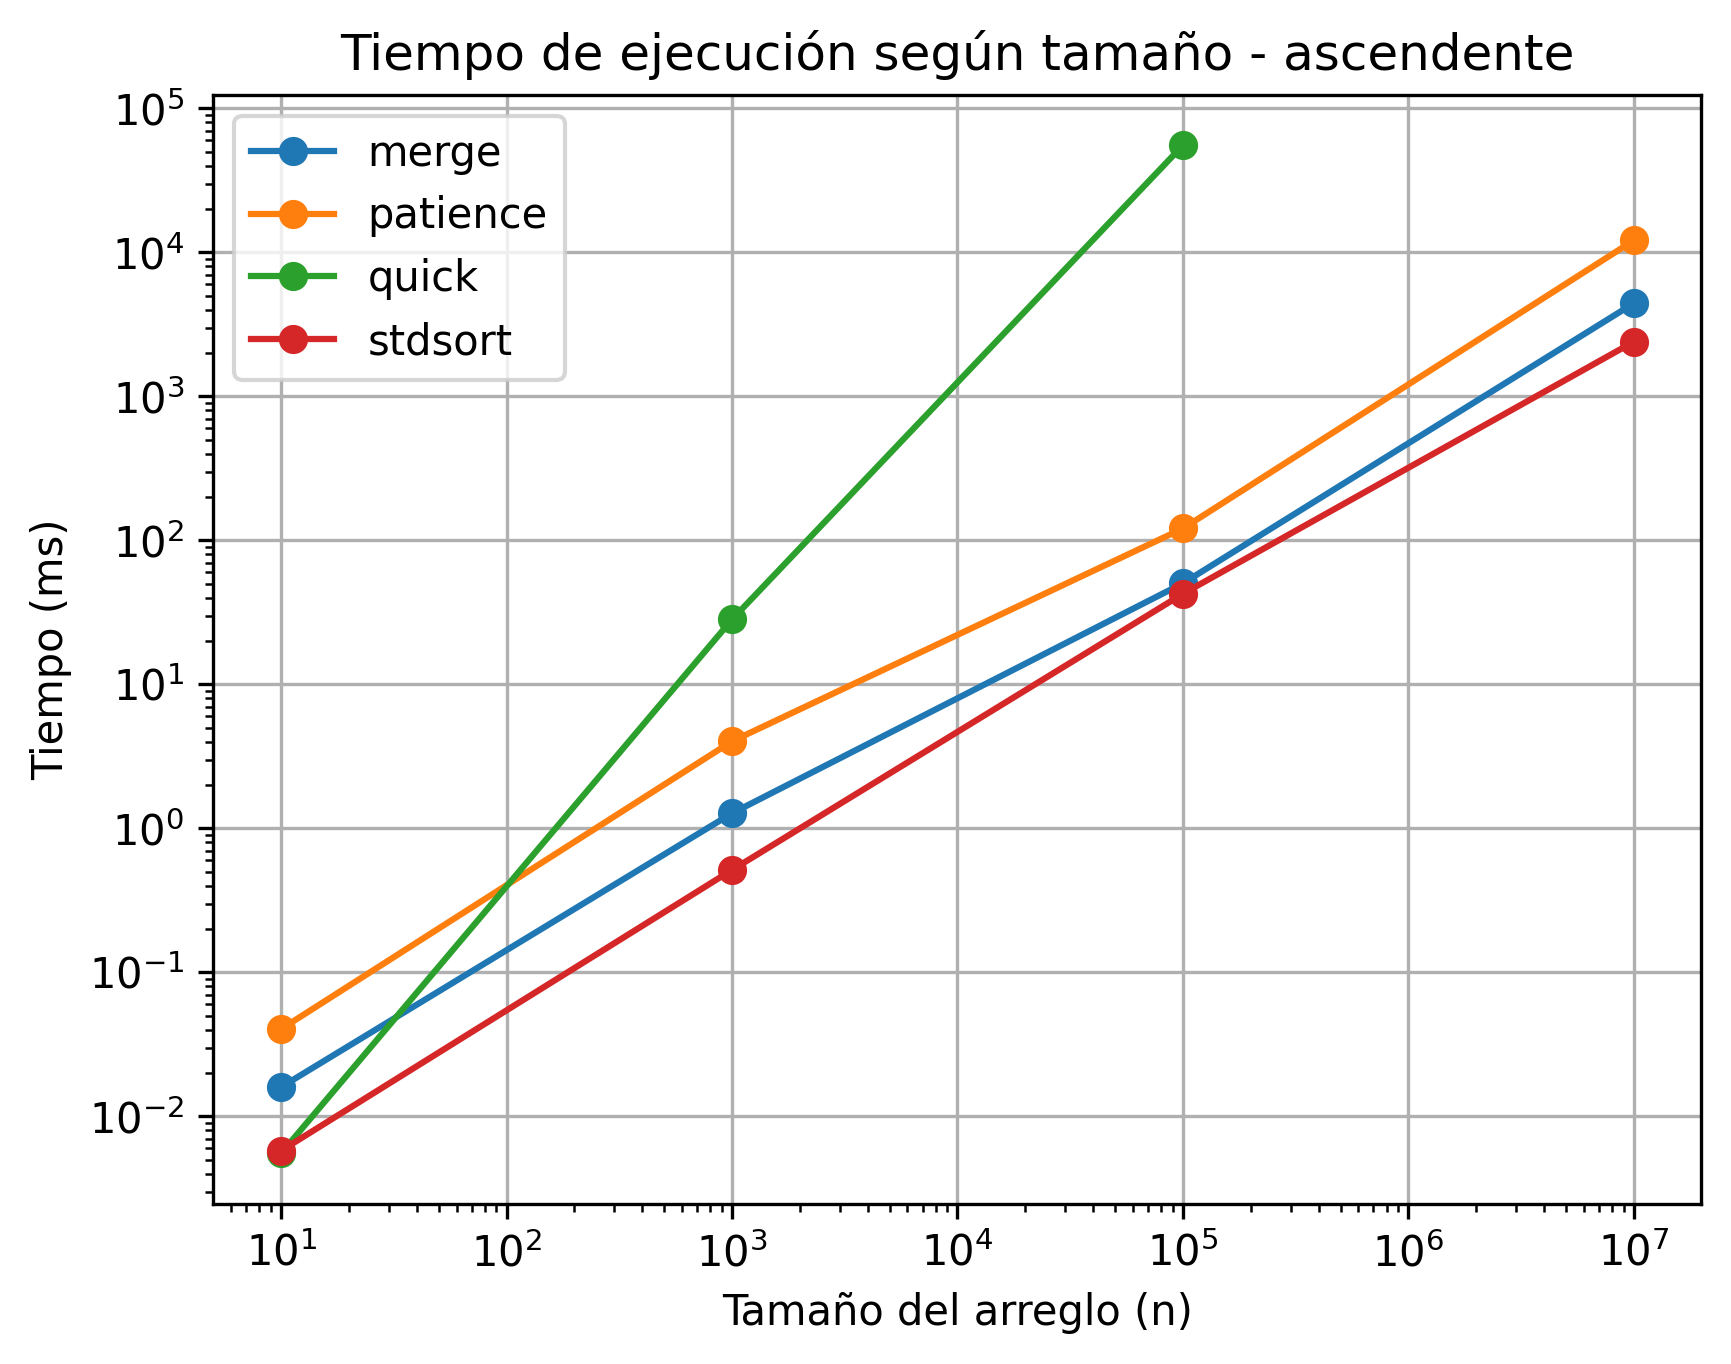
\includegraphics[width=0.48\textwidth]{../code/sorting/data/plots/sorting_tiempo_vs_n_ascendente.png}
    \caption{Tiempos de ejecución según tamaño de entrada (escala log-log). Izquierda: Arreglos aleatorios. Derecha: Arreglos ascendentes.}
    \label{fig:sorting_growth}
\end{figure}

En la Figura \ref{fig:sorting_growth}, se confirma que todos los algoritmos presentan una tendencia lineal-logarítmica. Las líneas mantienen pendientes similares; la diferencia principal radica en su desplazamiento vertical, el cual está determinado por el entorno sobre el cual se ejecuta el experimento y su propia gestión de los recursos computacionales.

\subsection{Multiplicación de Matrices}

Para la multiplicación de matrices, la Tabla \ref{tab:matrix_summary} muestra los tiempos obtenidos en el dominio máximo evaluado ($n=256$). 

\begin{table}[H]
\centering
\caption{Tiempo de ejecución promedio (ms) para $n=256$.}
\label{tab:matrix_summary}
\begin{tabular}{lrrr}
\hline
\textbf{Algoritmo} & \textbf{Densa} & \textbf{Diagonal} & \textbf{Dispersa} \\
\hline
Naive & 472.93 & 470.43 & 486.41 \\
Strassen & 15679.18 & 15765.45 & 15860.05 \\
\hline
\end{tabular}
\end{table}

A diferencia del caso de ordenamiento, la topología de la matriz (densa, diagonal o dispersa) no generó diferencias significativas de tiempo intragrupo. Sin embargo, el contraste entre algoritmos es drástico: el enfoque clásico (Naive) es más de 30 veces más rápido que Strassen para $n=256$.

Este fenómeno se visualiza claramente en la Figura \ref{fig:matrix_growth}, donde graficamos la curva de crecimiento temporal de ambos métodos.

\begin{figure}[H]
    \centering
    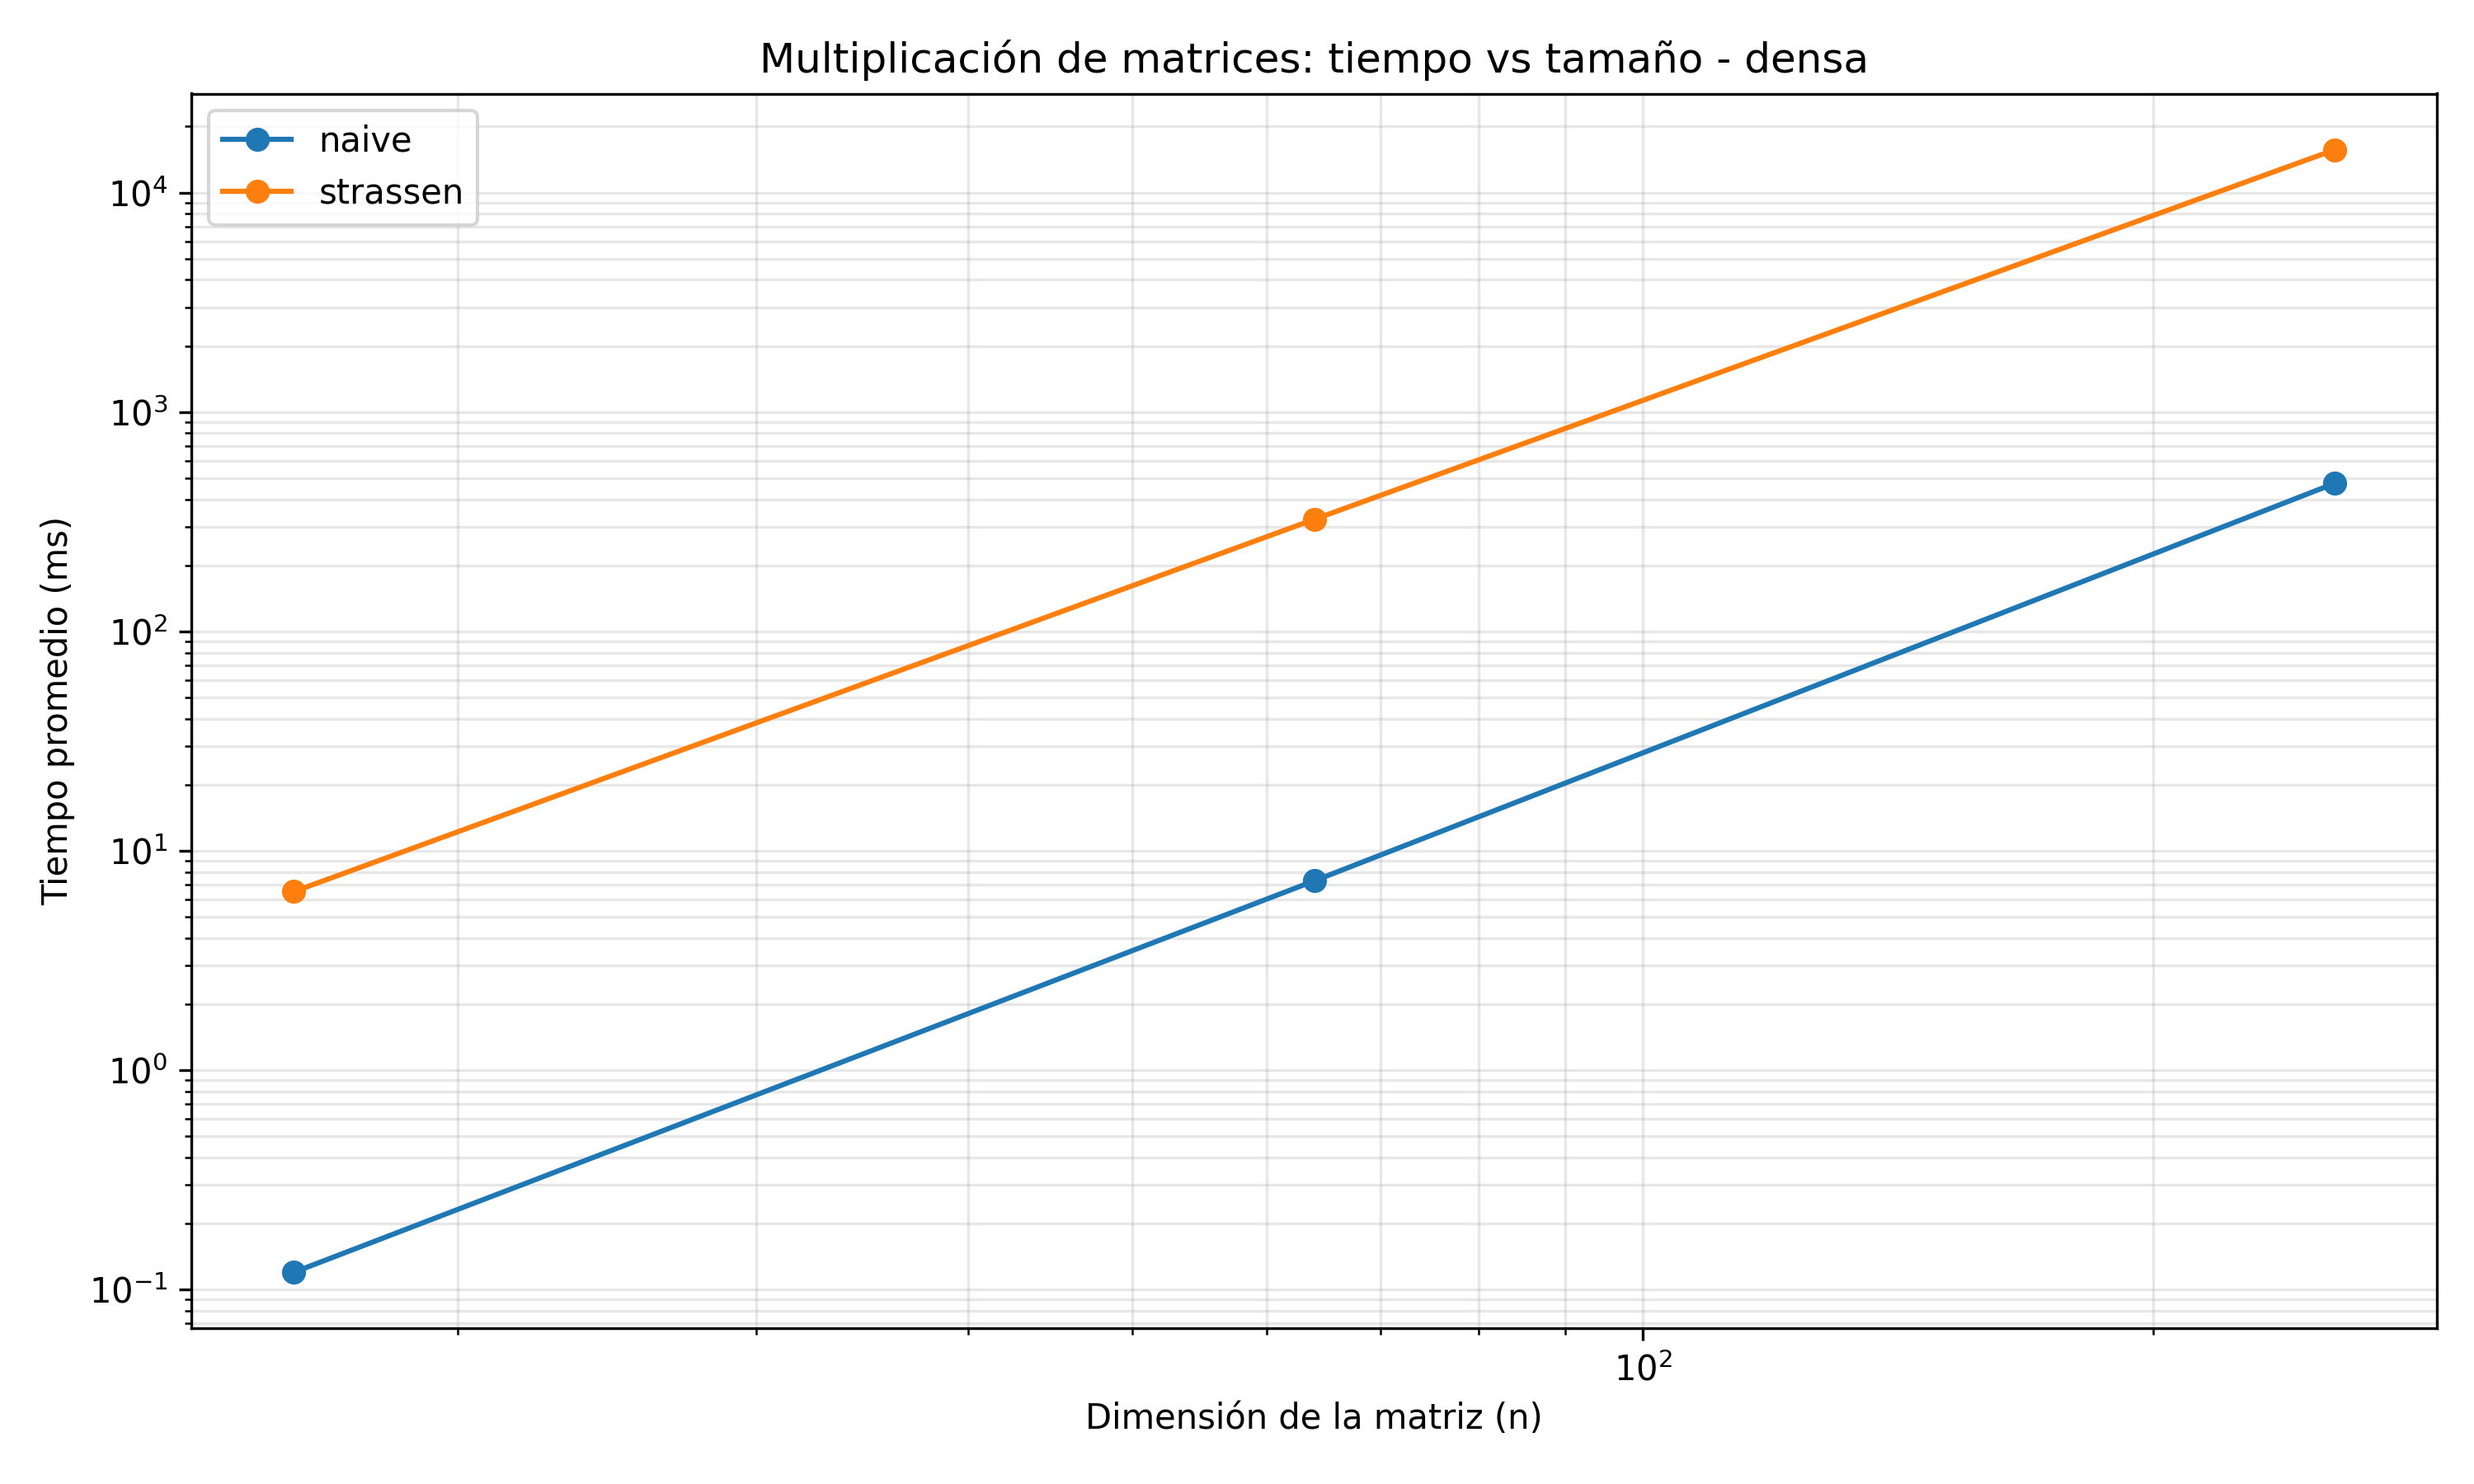
\includegraphics[width=0.6\textwidth]{../code/matrix_multiplication/data/plots/matrix_multiplication/tiempo_ms_vs_n_densa.png}
    \caption{Tiempo de ejecución versus dimensión de la matriz ($n$) para matrices densas.}
    \label{fig:matrix_growth}
\end{figure}

La Figura \ref{fig:matrix_growth} evidencia que el manejo de la reserva de memoria, copias de sub-arreglos y las llamadas recursivas son masivas. Hasta el dominio evaluado de $n=256$, la ventaja del exponente asintótico no es capaz de compensar el peso operativo, demostrando que Strassen solo sería práctico cruzando un umbral de $n$ considerablemente mayor.